%==============================================================================%
%                PRØVE | FORKURS 1P-2P LÆRERUTDANNING | V2017                  %
%==============================================================================%
%
% __/\\\\\\\\\\\\____________________/\\\\\\___________________/\\\_
%  _\/\\\////////\\\_________________\////\\\_______________/\\\\\\\_
%   _\/\\\______\//\\\___________________\/\\\______________\/////\\\_
%    _\/\\\_______\/\\\_____/\\\\\\\\_____\/\\\__________________\/\\\_
%     _\/\\\_______\/\\\___/\\\/////\\\____\/\\\__________________\/\\\_
%      _\/\\\_______\/\\\__/\\\\\\\\\\\_____\/\\\__________________\/\\\_
%       _\/\\\_______/\\\__\//\\///////______\/\\\__________________\/\\\_
%        _\/\\\\\\\\\\\\/____\//\\\\\\\\\\__/\\\\\\\\\_______________\/\\\_
%         _\////////////_______\//////////__\/////////________________\///_
%
%==============================================================================%
%                              UTEN HJELPEMIDDEL                               %
%==============================================================================%

\Del{u}

% ==============================================================================

\Oppgave[5] % Oppgave 1.1

I \cref{table:del-1-oppgave-1.1} ser du hvor mange ganger Inger har vært på
trening hver uke de $12$ siste ukene.\\

\begin{table}[H]
  \caption{}
  \label{table:del-1-oppgave-1.1}
  \begin{tabularx}{\textwidth}{*{12}{Y}} \hline
    4 & 5 & 5 & 5 & 2 & 0 &
    1 & 1 & 3 & 5 & 6 & 5 \\ \hline
  \end{tabularx}
\end{table}

\begin{oppgaver}
  \Item{1} Bestem medianen, gjennomsnittet, typetallet og variasjonsbredden
    for dette datamaterialet.
\end{oppgaver}

\begin{oppgaver}
  \Item{2} Sett opp en tabell som viser frekvens og kumulativ frekvens for
    antall treninger hver uke.
\end{oppgaver}

\begin{oppgaver}
  \Item{1} Hva forteller den kumulative frekvensen for fire treninger hver
    uke?
\end{oppgaver}

% ==============================================================================

\Oppgave[1] % Oppgave 1.2
\points*{1}

Regn ut og skriv svaret på standardform
%
\begin{equation*}
  \SI{2.5e-15}{}
  \cdot
  \SI{0.00006}{}
\end{equation*}

% ==============================================================================

\Oppgave[2] % Oppgave 1.3
\points*{2} %

Caffè latte er en kaffedrikk som lages av espresso og melk.
Forholdet mellom espresso og melk er vanligvis $1\colon3$. \medskip

Hvor mange desiliter melk trenger du for å lage \SI{3}{\deci\liter} caffè latte?

% ==============================================================================

\Oppgave[2] % Oppgave 1.4
\points*{2} %

En vare kostet $480$ kroner i $2016$. Indeksen for denne varen var da $120$.
Anta at indeksen for varen vil være $96$ i $2020$.
Hva vil varen da koste i $2020$?

% ==============================================================================

\Oppgave[4] % Oppgave 1.5

\Cref{fig:Del-1-Oppgave-5-1} viser et trapes $ABCD$. $M$ er midtpunkt på $AB$. I
trapeset er det innskrevet en halvsirkel som har $DC$ som diameter og går
gjennom $M$. $AM = DC = 2$.

\begin{figure}[H]
  \tikzsetnextfilename{Forkurs-1p-2p-laererutdanning-2017-V-oppgave-1-5}
  \begin{tikzpicture}[inner sep=0,outer sep=0, minimum size=0pt]
    \def\AM{4}\def\DC{\AM}\def\nodeDist{0.25}

    \coordinate[label={[label distance=\nodeDist cm]225:A}] (A) at (0,0);
    \coordinate[label={[label distance=\nodeDist cm]270:M}] (M) at (\AM,0);
    \coordinate[label={[label distance=\nodeDist cm]315:B}] (B) at (2*\AM,0);

    \coordinate[label={[label distance=\nodeDist cm]45:C}] (C) at (1.5*\AM,0.5*\AM);
    \coordinate[label={[label distance=\nodeDist cm]135:D}] (D) at (0.5*\AM,0.5*\AM);

    \draw[thick, maincolorDark, fill = maincolorLight] (A) -- (B)-- (C) -- (D) -- cycle;
    \draw[thin, maincolorDark, fill = maincolorMedium] (C) -- (D) arc(180:360:0.5*\AM);
  \end{tikzpicture}
  \caption{}
  \label{fig:Del-1-Oppgave-5-1}
\end{figure}

\begin{oppgaver}
  \Item{2} Gjør beregninger og avgjør om arealet av halvsirkelen er større enn
    det samlede arealet av de lyse områdene.
\end{oppgaver}

\begin{losninger}
  La oss for enkelhetens skyld anta at $AM = DC = a$, hvor $a$ bare er ett
  positivt tall. Radiusen til halvsirken er halvparten av lengden $DC$ slik
  at arealet blir
  %
  \begin{equation*}
    A_{\text{halvsirkel}}
    = \frac{\pi (a/2)^2}{2}
    = \frac{\pi}{8} a^2
  \end{equation*}
  %
  For å bestemme arealet til trapset trenger vi høyden, men dette er jo bare
  radiusen til halvsirkelen $h = DC/2 = a/2$
  %
  \begin{equation*}
    A_{\text{trapes}}
    = \frac{|DC| + |AB|}{2} \cdot h
    = \frac{a + (2a)}{2} \cdot \frac{a}{2}
    = \frac{3}{4}a^2.
  \end{equation*}
  %
  Det lyselilla området blir differansen mellom halvsirkelen og trapeset
  %
  \begin{equation*}
    A_{\text{lyselilla}}
    = A_{\text{trapes}} - A_{\text{halvsirkel}}
    = \frac{3}{4}a^2 - \frac{\pi}{8} a^2.
  \end{equation*}
  %
  For å finne ut hvilke området som har størst areal kan vi se at
  %
  \begin{equation*}
    A_{\text{lyselilla}}
    = \frac{3}{4}a^2 - \frac{\pi}{8} a^2
    < \frac{\pi}{4}a^2 - \frac{\pi}{8} a^2
    = \frac{\pi}{8} a^2
    =  A_{\text{halvsirkel}}
  \end{equation*}
  %
  slik at arealet til de lyselilla området er mindre enn halvsirkelen.
\end{losninger}

\begin{oppgaver}
  \Item{2} Vis at omkretsen av trapeset er $6 + 2\sqrt{2}$.
\end{oppgaver}

\begin{losninger}
  Omkretsen til trapeset er gitt som
  %
  \begin{equation}
    O_{\text{trapes}} = |AB| + |BC| + |CD| + |DA|
  \end{equation}
  %
  Hvor det bare er lengdene $|CD|$ og $|DA|$ som er ukjente. La oss først
  finne $|DA|$ vi merker oss først at lengden $|AE| = a/2$ siden $|AE| = |AM|
  - |DM'| = a - a/2$.  Tilsvarende så er $|DE| = a/2$. Fra pytagoras har vi at
  %
  \begin{equation}
    |AD|
    = \sqrt{|AE|^2 + |DE|^2}
    = \sqrt{(a/2)^2 + (a/2)^2}
    = \sqrt{2}a/2
  \end{equation}
  %
  Fra symmetri så er $|BC|=|AD|$ slik at omkretsen blir
  %
  \begin{align*}
    O_{\text{trapes}}
        & = |AB| + |BC| + |CD| + |DA| \\
        & =   2a  +   \frac{\sqrt{2}}{2}a + a + \frac{\sqrt{2}}{2}a
        =   3a  + \sqrt{2}a
  \end{align*}
  %
  ved å sette inn $a=2$ får vi $O_{\text{trapes}} = 6 + 2 \sqrt{2}$ som var
  det vi ønsket å vise.
\end{losninger}

% ==============================================================================

\Oppgave[2] % Oppgave 1.6

Thomas kjøpte en tre år gammel bruktbil for $\num{200000}$ kroner i $2017$. Han
antar at bilens verdi vil avta med  $\SI{10}{\percent}$ per år framover.

\begin{oppgaver}
  \Item{1} Hvilken av grafene $f$, $g$ og $h$ i koordinatsystemet i
    \cref{fig:del-1-oppgave-6} viser hvordan bilens verdi vil endre seg de neste
    åtte årene dersom Thomas har rett? Begrunn svaret ditt.
\end{oppgaver}

\begin{figure}[H]
  \tikzsetnextfilename{Forkurs-1p-2p-laererutdanning-2017-V-oppgave-1-6}
  \begin{tikzpicture}
    \begin{axis}[
      Eksamen1,
      ytick={0,2,...,20},
      yticklabel = {\num{\fpeval{\tick*10000}}},
      xtick={0,1,...,8},
      ymin=-.1,
      ymax=23,
      xmin=-.1,
      xmax=9,
      domain = 0:8,
      ]
      \addplot[color=maincolorMedium!30!white,thick,samples=50] {20-2*x} node[above,pos=1] {$g$};
      \addplot[color=maincolorMedium,thick,samples=50] {20*e^(-0.2*x)} node[below,pos=0.5] {$h$};
      \addplot[color=maincolorMedium!30!black,thick,samples=50] {20*0.9^x} node[above,pos=0.6] {$f$};
      \node[] at (axis cs: 2.5,21) {bilens verdi (kroner)};
      \node[] at (axis cs: 7,1.5) {År etter 2017};
    \end{axis}
  \end{tikzpicture}
  \caption{}
  \label{fig:del-1-oppgave-6}
\end{figure}

Anta at bilens verdi har avtatt med $\SI{15}{\percent}$ per år fra den var ny,
og fram til Thomas kjøpte den.

\begin{oppgaver}
  \Item{1} Sett opp et uttrykk som Thomas kan bruke for å regne ut hvor mye
    bilen var verdt da den var ny.
\end{oppgaver}

% ==============================================================================

\Oppgave[4] % Oppgave 1.7

Et firma selger postkassestativ og postkasser.

\begin{itemize}
  \item Petter og naboene hans kjøpte ett postkassestativ og tre like
    postkasser. De betalte til sammen $\num{12850}$ kroner.
    %
  \item Morten og naboene hans kjøpte ett postkassestativ og seks like
    postkasser. De betalte til sammen $\num{19000}$ kroner.
\end{itemize}

\begin{oppgaver}
  \Item{1} Hvor mye koster ett postkassestativ, og hvor mye koster én
    postkasse?
\end{oppgaver}

\begin{oppgaver}
  \Item{1} Bestem en lineær modell som viser sammenhengen mellom antall
    postkasser og samlet pris for stativet og postkassene.
    \label{oppgave:del-1-oppgave-7b}
\end{oppgaver}

\begin{oppgaver}
  \Item{2} Bruk modellen fra \cref{oppgave:del-1-oppgave-7b} til å bestemme
    prisen for et stativ med åtte postkasser.
\end{oppgaver}

\begin{center}
  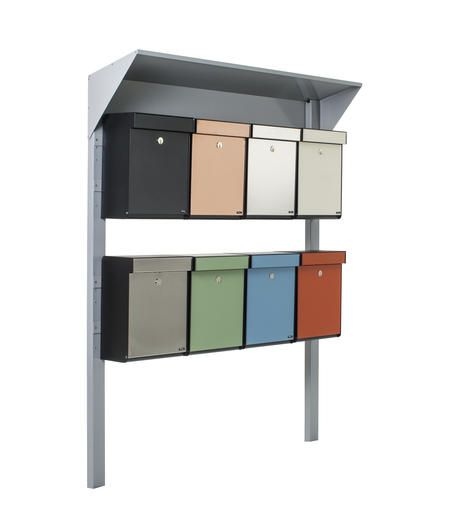
\includegraphics[scale=0.5]{postkasse.jpg}
\end{center}

% ==============================================================================

\Oppgave[2] % Oppgave 1.8
\points*{2}

I en bolle med gullfisk er det $\SI{25}{\percent}$ av typen Oranda. Det blir så
sluppet oppi like mange nye fisker av typen Oranda som det var der fra før.
\medskip

Hvor mange prosent av gullfiskene i bollen er nå av typen Oranda?

\begin{center}
  \tikz\node[circle,draw,fill=black,
  text=white,
  path picture={
    \node at (path picture bounding box.center){
      \includegraphics[width=4cm]{oranda.jpg}
    };
  }]{\phantom{heeelllo0000000000}};
\end{center}

% ==============================================================================

\Oppgave[2] % Oppgave 1.9
\points*{2}

Ved en skole ble $\num{155}$ tilfeldige elever spurt om reisetid i minutter fra
bosted til skole. Se \cref{table:del-1-oppgave-1.9}.

\begin{table}[H]
  \caption{}
  \label{table:del-1-oppgave-1.9}
  \begin{tabular}{|c | S[table-format=3.0]|}
    \tableHeaders{Reisetid i minutt}{Frekvens}
    $\left[\phantom{1}0, 10 \right\rangle$ & 25 \\
    $\left[10, 20 \right\rangle$ & 50 \\
    $\left[20, 40 \right\rangle$ & 60 \\
    $\left[40, 80 \right\rangle$ & 20 \\
    \tableHeaders{Totalt}{155}
  \end{tabular}
\end{table}

Bestem medianen for datamaterialet.

% ==============================================================================
